\section{Data Processing Pipeline}

Baihu converts heterogeneous human-teleoperated robot operation records into a consistent dataset for large-scale policy training. The source trajectories are stored in HDF5 format and are standardized into LeRobot v2.1 for downstream imitation-learning and vision-language-action training. The processing pipeline emphasizes three requirements: preserving embodiment-specific control information, filtering invalid or task-inconsistent trajectories, and producing a unified representation that can be loaded by modern robot learning systems.

\subsection{HDF5 ingestion and trajectory validation}

Raw Baihu trajectories are first organized as HDF5 records. Each record is associated with a robot platform, task identity, episode identity, and available modality fields. Depending on the source platform and task setup, a trajectory may include visual observations, robot proprioceptive states, robot actions, task annotations, timestamps, and episode-level metadata.

Because Baihu integrates data from multiple robot platforms, validation is required before data enters the released training corpus. The pipeline checks whether each episode contains temporally ordered observations and actions, usable modality fields, consistent task metadata, valid platform information, and aligned observation-action sequences. This validation step removes incomplete, corrupted, or unusable trajectories that would otherwise provide incorrect supervision during model training.

\subsection{Quality control and metadata standardization}

Baihu uses a multi-stage quality control workflow covering data acquisition, monitoring, upload, validation, cleaning, review, and final delivery. This workflow is important at the scale of Baihu because even a small fraction of invalid trajectories can correspond to a large amount of unusable data. Quality control therefore aims to maintain consistency across heterogeneous platforms while preserving the diversity needed for embodied model pretraining.

A trajectory is retained only when it satisfies the task request under which it was collected. Trajectories that do not follow the task requester specification are removed from the dataset. Typical removal cases include incorrect scene setup, incorrect objects or tools, wrong manipulation procedure, incomplete task execution, corrupted recordings, missing modality fields, inconsistent task metadata, or misaligned observation-action sequences. As a result, Baihu does not intentionally preserve failed or task-inconsistent demonstrations as training examples in the released corpus.

Task and episode metadata are standardized to support dataset analysis and model conditioning. Each episode is associated with task information, platform metadata, and source-specific fields when available. These annotations enable analysis by task and platform, and they also provide the language or semantic conditioning signals used by vision-language-action policies. Since task annotations are manually provided when collection requirements are proposed, metadata standardization also checks that the recorded trajectory remains consistent with the intended task description.

\subsection{State and action schema alignment}

State and action representations differ across robot platforms. Platforms may have different joint layouts, gripper or hand structures, control frequencies, and action semantics. Baihu therefore preserves platform-specific schemas that define which dimensions correspond to arm joints, grippers, hands, or other controllable components.

This schema alignment is important for both training and evaluation. It allows each platform to retain its native control representation while enabling unified dataset loading. It also supports metric definitions such as Joint MSE and ALL MSE: Joint MSE uses only joint-related action dimensions, while ALL MSE uses the full action vector for each platform.

For grippers and hands, values are stored according to the actual physical travel range of each platform. Baihu does not impose a single universal gripper or hand scale across robots. This design keeps the stored action values faithful to the original robot control space and avoids forcing heterogeneous end-effectors into an artificial shared range.

\subsection{HDF5-to-LeRobot v2.1 conversion}

After validation and schema alignment, Baihu is converted from the source HDF5 records into the LeRobot v2.1 format. The conversion standardizes episode and frame organization, synchronized visual observations, robot states, actions, human-provided task annotations, and episode-level metadata. This separates the source storage format from the model-training representation: HDF5 provides the original trajectory container, while LeRobot v2.1 provides a consistent interface for dataset loading, episode management, and downstream training.

Because the robot platforms have different embodiments and control spaces, Baihu does not force all platforms into an identical observation or action vector. Instead, each platform retains its modality-specific state, action, and camera schema within the shared LeRobot v2.1 interface. This design enables consistent data access across platforms while preserving the physical control semantics of each robot.

\section{Benchmark Experiments}

To demonstrate the value of Baihu for embodied foundation model training, we evaluate whether a model trained on Baihu improves offline action prediction on external evaluation datasets. The datasets used for open-loop evaluation are not part of the Baihu training corpus. The benchmark therefore measures transfer from Baihu pretraining to held-out evaluation trajectories collected separately from Baihu.

\subsection{Offline open-loop zero-shot evaluation}

Open-loop evaluation provides an offline assessment by comparing the model's predicted actions against reference actions from human-teleoperated robot demonstrations. In this benchmark, we compare a no-training GR00T N1.6 checkpoint~\cite{nvidia2025grootn1}, checkpoint-1, with checkpoint-390000, which was trained on Baihu for one epoch. The evaluation covers \textbf{13 platforms} and \textbf{42 paired task-dataset records} drawn from datasets that are external to Baihu and excluded from Baihu training. No additional finetuning is performed on these evaluation datasets. We therefore use zero-shot to denote dataset-level transfer from Baihu pretraining to external held-out evaluation data.

\subsection{Evaluation protocol}

For each task-dataset record, five trajectories are randomly sampled from the corresponding external evaluation dataset. The same sampled trajectories are then used to evaluate both checkpoints, providing a paired comparison between the no-training baseline and the Baihu-trained model. The model predicts actions from the recorded observations of each trajectory, and the prediction error is measured against the associated human-teleoperation actions. Predictions are generated with an action horizon of 30, and each trajectory is evaluated over its available length up to a maximum of 3000 steps. The task-level result is obtained by averaging the trajectory-level MSE values over the five trajectories.

Per-platform results are computed as the unweighted mean over the task-dataset records associated with each platform. The overall benchmark result is then reported as the unweighted mean across all 42 paired task-dataset records. This evaluation design gives each task-dataset record equal weight, independent of the amount of data available for a particular platform or task.

\subsection{Evaluation metrics}

All reported MSE values are normalized by action range to make errors more comparable across platforms with different action scales. For a trajectory with $T$ evaluated timesteps and a selected set of $D$ action dimensions, the normalized MSE is defined as

\begin{equation}
\mathrm{NMSE}
=
\frac{1}{TD}
\sum_{t=1}^{T}
\sum_{d=1}^{D}
\left(
\frac{\hat{a}_{t,d}-a_{t,d}}
{a_{d}^{\max}-a_{d}^{\min}}
\right)^{2},
\label{eq:normalized-mse}
\end{equation}

where $a_{t,d}$ and $\hat{a}_{t,d}$ denote the reference and predicted action values for dimension $d$ at timestep $t$, respectively, and $a_{d}^{\max}-a_{d}^{\min}$ is the corresponding action range. The same action normalization statistics are used for checkpoint-1 and checkpoint-390000, ensuring that the two checkpoints are compared under an identical metric scale.

\textbf{Normalized ALL MSE} is used as the primary evaluation metric. In Eq.~\ref{eq:normalized-mse}, $D$ includes the complete action vector, consisting of robot joint actions and end-effector actuation dimensions such as grippers or dexterous hands.

\textbf{Normalized Joint MSE} is reported as an auxiliary diagnostic metric. In this case, $D$ includes only robot joint action dimensions and excludes end-effector actuation dimensions, which may correspond to a gripper or a dexterous hand depending on the platform. This separation enables joint-motion prediction to be analyzed independently from platform-specific end-effector control.

\subsection{Overall results}

The benchmark results show that one epoch of training on Baihu substantially reduces normalized offline open-loop prediction error across the 13 evaluated platforms and 42 external paired task-dataset records. At the aggregate level, the Baihu-trained checkpoint reduces Normalized ALL MSE from 0.157283 to 0.005051, corresponding to a \textbf{96.79\%} relative improvement. It also reduces Normalized Joint MSE from 0.116746 to 0.000680, corresponding to a \textbf{99.42\%} relative improvement. The per-platform comparisons are visualized in Fig.~\ref{fig:per-platform-zero-shot}.

This indicates that Baihu provides effective supervision for improving full-vector and joint-related action prediction on evaluation data that were not included in the Baihu training corpus.

\subsection{Per-platform results}

Because Baihu is a multi-embodiment dataset, aggregate metrics alone are insufficient. We therefore also analyze the results separately for each evaluated platform. Across all 13 platforms, the Baihu-trained checkpoint achieves lower Normalized ALL MSE and Normalized Joint MSE than the no-training baseline.

\begin{figure}[t]
\centering
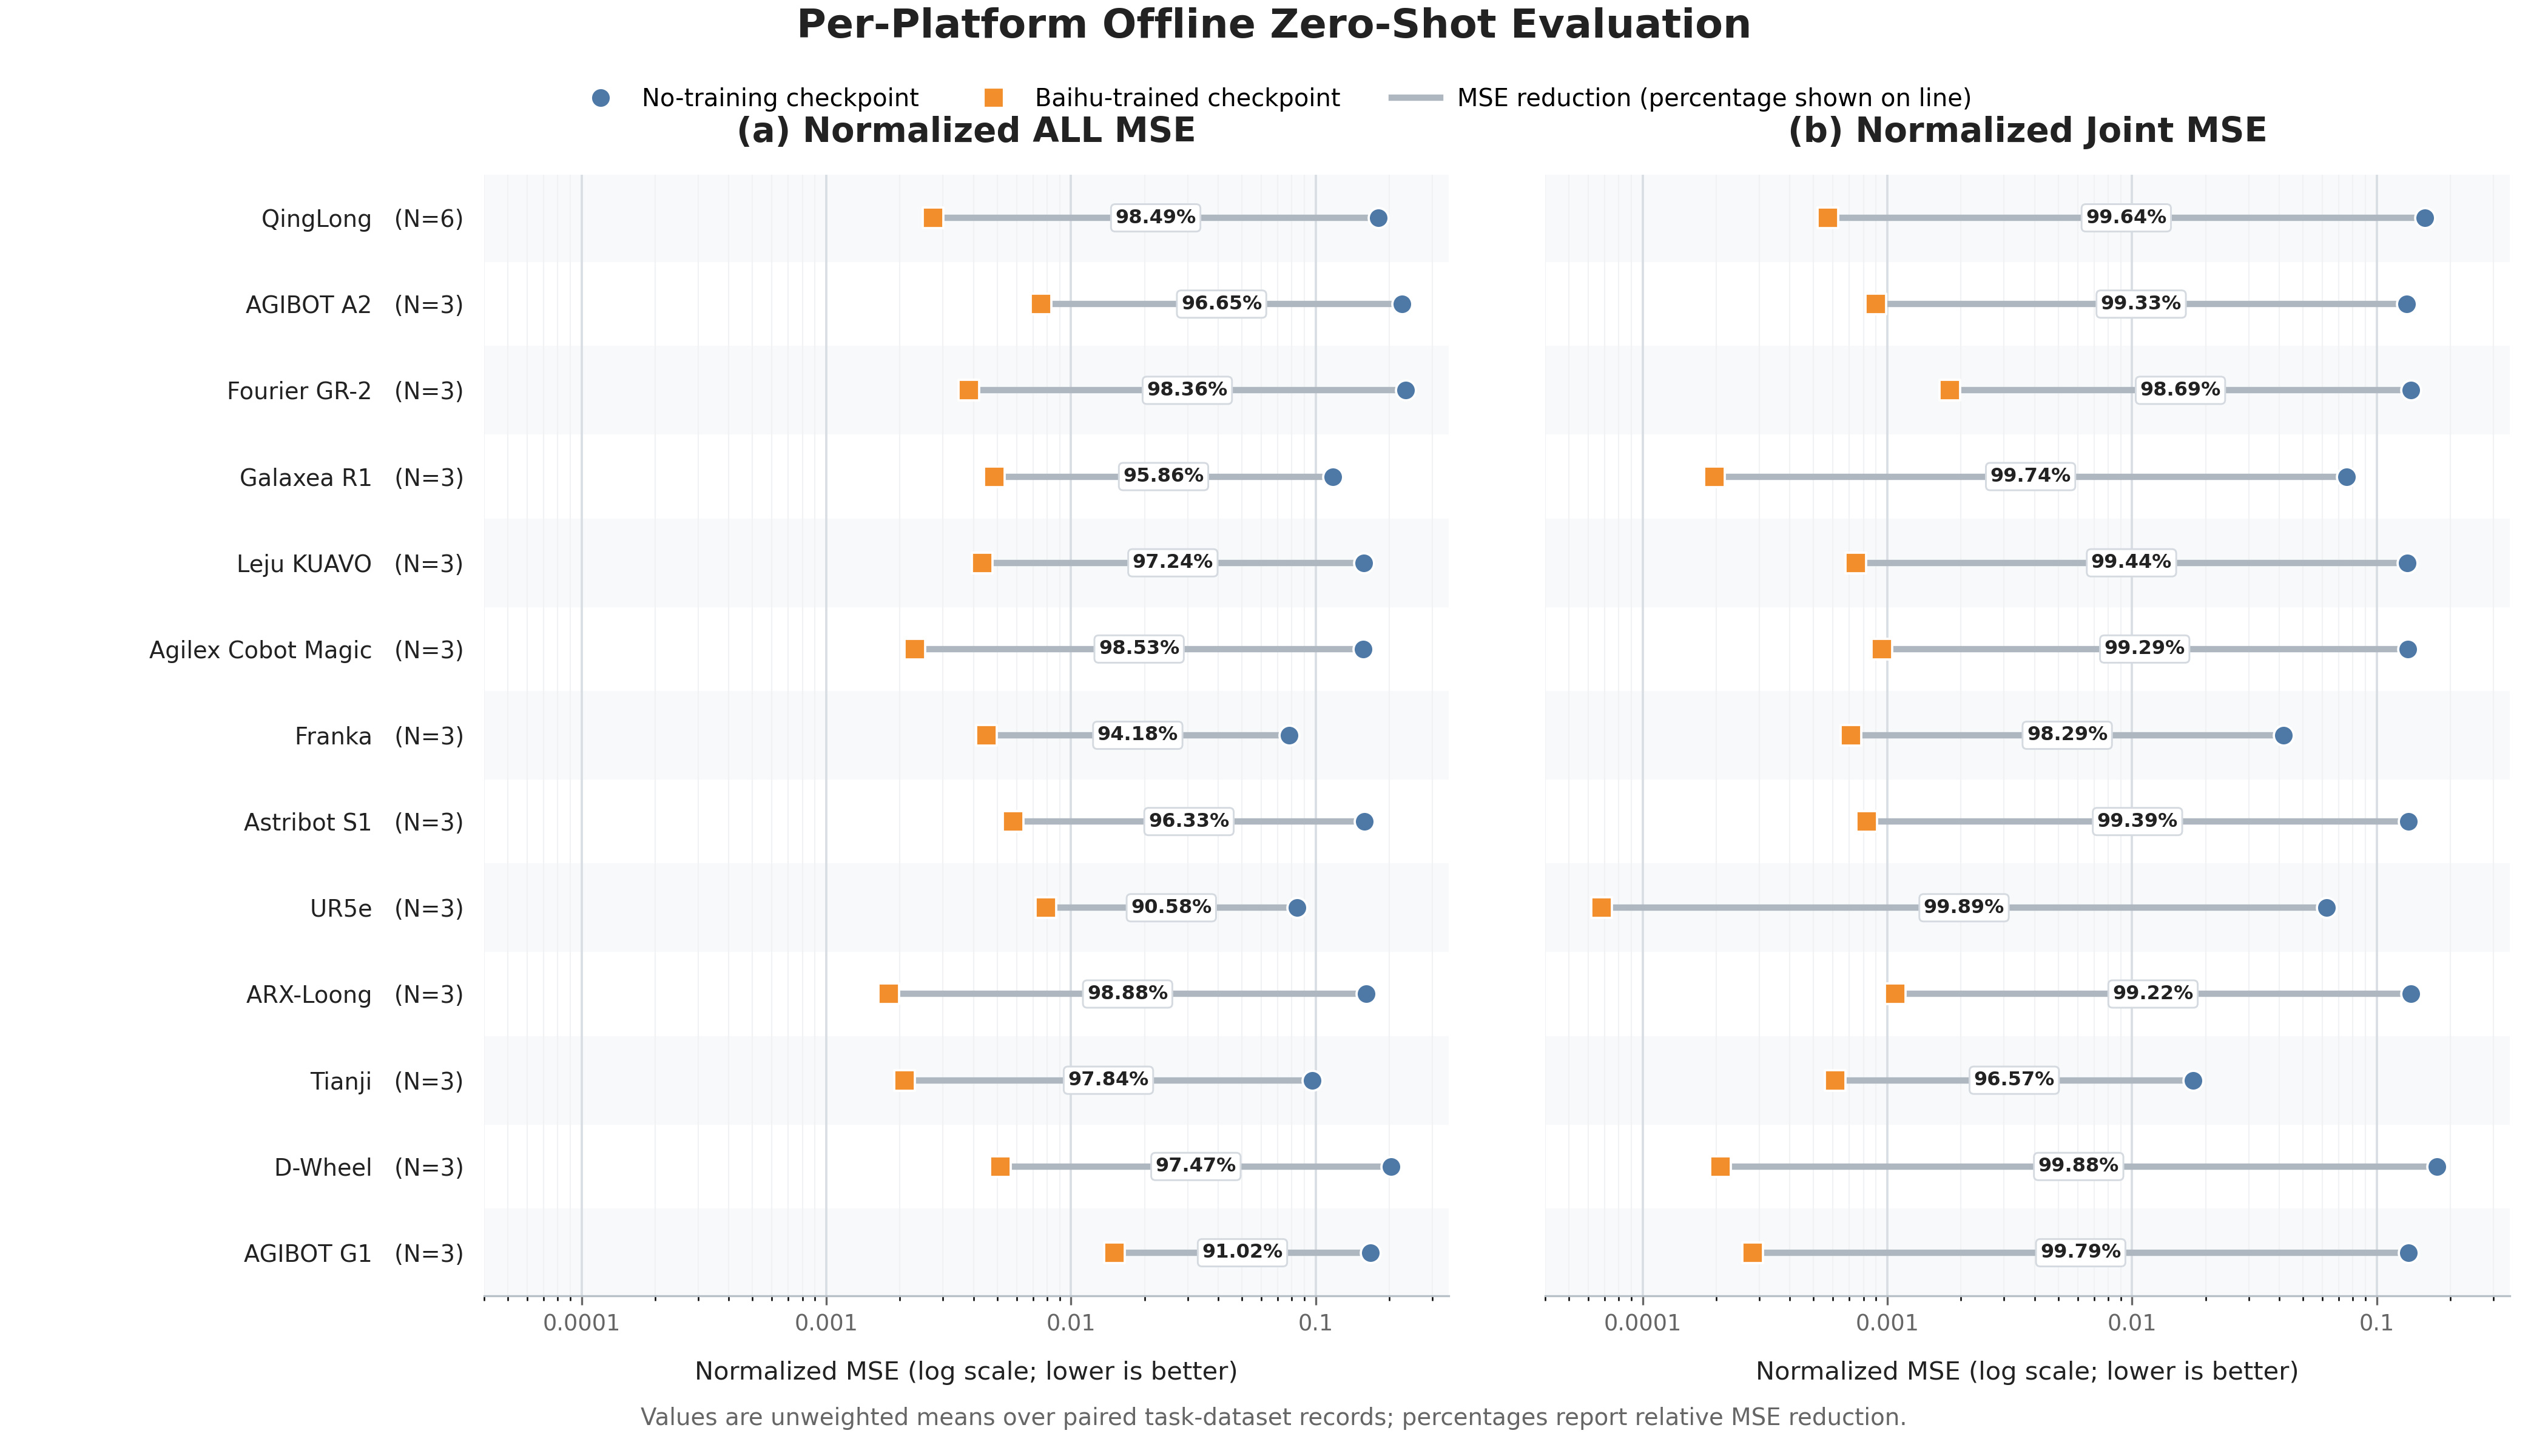
\includegraphics[width=\textwidth]{figures/per_platform_zero_shot_dumbbell.jpg}
\caption{Per-platform offline zero-shot evaluation on datasets external to Baihu. Each row compares the no-training GR00T N1.6 checkpoint (checkpoint-1) with the checkpoint trained on Baihu for one epoch (checkpoint-390000) for Normalized ALL MSE and Normalized Joint MSE. Connected markers show the change after Baihu training; lower is better. Each platform value is the unweighted mean over its paired task-dataset records. QingLong contains six records, while each of the remaining platforms contains three.}
\label{fig:per-platform-zero-shot}
\end{figure}

Figure~\ref{fig:per-platform-zero-shot} shows that the improvement is consistent rather than being driven by a small subset of embodiments. Relative reductions range from 90.58\% to 98.88\% for Normalized ALL MSE and from 96.57\% to 99.89\% for Normalized Joint MSE. Joint prediction improves particularly uniformly across platforms, whereas the remaining ALL MSE varies more because it additionally includes platform-specific end-effector dimensions such as grippers and dexterous hands. These results support the use of Baihu as a shared pretraining corpus for heterogeneous robot embodiments.

\subsection{Task-level analysis}

Task-level results further show that Baihu training improves normalized offline prediction across the 42 external paired task-dataset records. Task-level reporting is especially useful because different platforms may have different action spaces, control frequencies, and end-effector structures.

Table~\ref{tab:task-level} reports Normalized ALL MSE, Normalized Joint MSE, and relative improvement for each of the 42 paired task-dataset records. The full task-level table is provided in Appendix~\ref{app:task-level}.

The strongest improvements are observed on records where the no-training checkpoint has relatively large action prediction error. The remaining residual errors after Baihu training are small in absolute value, but they can still vary across platforms and tasks due to differences in action representation and task dynamics.

\subsection{Additional benchmark extensions}

The current benchmark provides a dataset-level held-out offline zero-shot comparison. Future versions can extend the benchmark with data-scaling evaluation, held-out platform evaluation, closed-loop simulation evaluation, and real-world rollout success rate.
